\subsection{复合积的七种计算}

设 M、M' 和 M'' 是三个左 A-模， \(a : R \to M\) , \(a' : R' \to M'\) 与 \(a'' : R'' \to M''\) 为投射分解， \(c : M \to E\) , \(c' : M' \to E'\) 与 \(c'' : M'' \to E''\) 为内射分解。由 X 第 100 页定理 1 及第 103 页命题 2 可知，图表：

\[
\begin{array}{c} \mathrm{H} (\operatorname{Homgr} _ {A} (M, E ^ {\prime})) \xrightarrow {} \mathrm{H} (\operatorname{Homgr} _ {A} (R, E ^ {\prime})) \xrightarrow {} \mathrm{H} (\operatorname{Homgr} _ {A} (R, M ^ {\prime})) \\ \uparrow \quad \xrightarrow {\varphi (M , E ^ {\prime})} \quad \downarrow \varphi (\mathbf {R}, E ^ {\prime}) \quad \uparrow \\ \mathrm{H} (\operatorname{Homgr} _ {A} (E, E ^ {\prime})) \xrightarrow {\varphi (E , E ^ {\prime})} \operatorname{Ext} _ {A} (M, M ^ {\prime}) \xleftarrow {\varphi (R , R ^ {\prime})} \mathrm{H} (\operatorname{Homgr} _ {A} (R, R ^ {\prime})) \end{array}
\]

（其中未标注的箭头由 \(c\) , \(a\) , \(c'\) , \(a'\) 典范地导出）是交换的，并且所有箭头都是同构，从而给出了关于 \(\mathrm{Ext}_{\mathbf{A}}(\mathbf{M}, \mathbf{M}')\) 的五种描述。类似地，可得到 \(\mathrm{Ext}_{\mathbf{A}}(\mathbf{M}', \mathbf{M}'')\) 的五个描述，以及 \(\mathrm{Ext}_{\mathbf{A}}(\mathbf{M}, \mathbf{M}'')\)

的同样多个描述。现在考虑七个复合同态

\[
\mathrm{H} \left(\operatorname{Homgr} _ {\mathbf {A}} \left(\mathrm{C} ^ {\prime}, \mathrm{C} ^ {\prime \prime}\right)\right) \otimes_ {k} \mathrm{H} \left(\operatorname{Homgr} _ {\mathbf {A}} \left(\mathrm{C}, \mathrm{C} ^ {\prime}\right)\right)\rightarrow \mathrm{H} \left(\operatorname{Homgr} _ {\mathbf {A}} \left(\mathrm{C}, \mathrm{C} ^ {\prime \prime}\right)\right),
\]

其中依次取(C, C', C'')为以下七个三元组：(R, R', R'')、(R, R', M'')、(R, R', E'')、(R, M', E'')、(R, E', E'')、(M, E', E'')、(E, E', E'')。

\pandocbounded{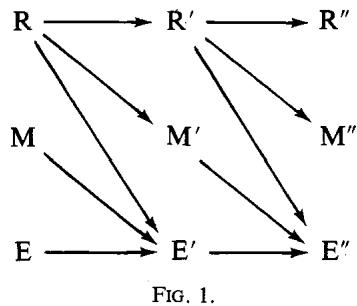
\includegraphics[keepaspectratio]{images/part001_66540ed3.jpg}}

通过上述同构，将H(Homgr \(_A\) (C, C'))等同于Ext (M, M')，同样地，将H(Homgr \(_A\) (C', C''))和H(Homgr \(_A\) (C, C''))也作相应等同，便得到七个同态。

\[
\operatorname{Ext} _ {\mathbf {A}} \left(\mathrm{M} ^ {\prime}, \mathrm{M} ^ {\prime \prime}\right) \otimes_ {k} \operatorname{Ext} _ {\mathbf {A}} \left(\mathrm{M}, \mathrm{M} ^ {\prime}\right)\rightarrow \operatorname{Ext} _ {\mathbf {A}} \left(\mathrm{M}, \mathrm{M} ^ {\prime \prime}\right).
\]

这七个同态彼此一致，并且与分解的选取无关。特别地，它们与第 2 号中通过三元组 (I(M), I(M'), I(M')) 所定义的同态一致。这确实可由将模 H(Homgr (C, C')) 解释为从复形 C 到 C' 的复形态射的同伦类所组成的模，以及以下事实得出：若在复形的一个图中

\[
\begin{array}{c} \mathrm{C} \xrightarrow {f} \mathrm{C} ^ {\prime} \xrightarrow {g} \mathrm{C} ^ {\prime \prime} \\ \alpha \Big \downarrow \qquad \qquad \alpha^ {\prime} \Big \downarrow \qquad \qquad \alpha^ {\prime \prime} \Big \downarrow \\ \mathrm{C} _ {1} \xrightarrow {f _ {1}} \mathrm{C} _ {1} ^ {\prime} \xrightarrow {g _ {1}} \mathrm{C} _ {1} ^ {\prime \prime} \end{array}
\]

\(\alpha'' \circ g\) 同伦于 \(g_1 \circ \alpha'\) ，而 \(\alpha' \circ f\) 同伦于 \(f_1 \circ \alpha\) ，则 \(\alpha'' \circ g \circ f\) 同伦于 \(g_1 \circ f_1 \circ \alpha\) （X，第 33 页，命题 4 及其推论）。

在下文中，我们将视情况使用上述七种复合同态构造中的某一种。

